% Chapter 1

\chapter{Introduzione} % Main chapter title

\label{Introduzione} % For referencing the chapter elsewhere, use \ref{Chapter1} 

\lhead{\emph{Introduzione}} % This is for the header on each page - perhaps a shortened title

%----------------------------------------------------------------------------------------

L’evoluzione di popolazioni di cellule proliferanti risulta spesso estremamente
difficile da caratterizzare mediante convenzionali tecniche di biologia
sperimentale \cite{bernitz2016stem}. Tuttavia, un’analisi approfondita di questi fenomeni
faciliterebbe lo studio e la comprensione di diverse patologie umane.
Per questa ragione, è necessario accoppiare metodologie computazionali 
avanzate ai classici esperimenti di laboratorio. Nel caso particolare della 
Leucemia Mieloide Acuta (LMA) si pensa che l'eterogeneità tra diverse 
sottopopolazioni cellulari presenti all'interno del tumore giochi un ruolo 
fondamentale per quanto riguarda la resistenza alle cure e il fatto che il 
tumore possa ripresentarsi a seguito del completamento della terapia 
\cite{dohner2015aml}.
Per lo studio di questo fenomeno si può optare per un approccio model-driven 
in modo da studiare le dinamiche riguardanti la proliferazione di 
popolazioni cellulari eterogenee \cite{aml2018unimib}. 
L'obiettivo di questo stage è lo sviluppo di un 
simulatore di divisione cellulare in grado di tenere conto della presenza 
di differenti tipi di popolazioni cellulari e della stocasticità degli eventi
di divisione ad essi correlati. Le cellule si divono in maniera esponenziale, 
quindi la simulazione di questi fenomeni comporta costi in termini di memoria 
e tempo esponenziali, infatti utilizzando un simulatore implementato 
solamente tramite sviluppo su Central Processing Unit (CPU) 
è emerso l'elevato costo 
computazionale necessario alla simulazione di popolazioni cellulari di grandi 
dimensioni. A causa di ciò si è reso necessario 
l'utilizzo di tecniche di accelerazione software per incrementare le 
performance del simulatore. Esistono diverse metodologie e architetture il cui 
obiettivo è l'incremento delle prestazioni dei software per cercare di ridurne
l'impatto in termini di costo computazionale di risorse sia fisiche, come la 
disponibilità di spazio di memorizzazione, sia temporali, ovvero il tempo 
necessario all'esecuzione del software. L'insieme di questi paradigmi 
costituisce l'High Performance Computing (HPC), solitamente utilizzato in 
ambito scientifico per ridurre i costi legati a simulazioni di natura 
biologica, chimica e fisica.
Generalmente all'interno di questa categoria possono essere distinti tre 
diversi tipi di architettura: il Computer cluster, il Grid computing e 
il General-Purpose computing on Graphics Processing Units (GPGPU).
Ognuna di queste architetture propone strategie differenti per quanto riguarda 
la risoluzione delle problematiche precedentemente elencate.
\\
Nei Computer cluster le elaborazioni sono svolte da CPU singole
(denominate nodi) e distribuite su macchine di elaborazione fisicamente 
differenti, come si può evincere dalla Figura \ref{fig:cluster-grid} 
e utilizzano una rete locale per comunicare tra di loro. Questi cluster
generalmente sono collocati all'interno dello stesso luogo
(una stanza o un intero edificio), risentono dunque solamente del ritardo generato
da una rete locale di computer. Solitamente questi cluster vengono utilizzati 
per simulazioni che necessitano di enormi quantità di dati per essere svolte, 
dunque la simulazione della proliferazione 
cellulare sarebbe uno spreco di risorse di elaborazione nel momento in cui i 
dati di input sono dell'ordine dei megabyte (MB).
\\
Il Grid computing mostrato in Figura \ref{fig:cluster-grid}
prevede che diversi enti ed organizzazioni mettano in condivisione risorse e
dati per portare a termine la medesima finalità.
I nodi delle risorse (sia hardware che softawre) possono essere
dislocati anche geografimente in luoghi differenti, 
il vantaggio è la disponibilità di grandi
quantità di dati e hardware per l'elaborazione degli stessi che non sarebbe
possibile ottenere utilizzando un'architettura Cluster. Anche in questo caso 
l'utilizzo di questa tipologia di elaborazione non è conveniente per la 
simulazione della proliferazione cellulare, poiché le informazioni necessarie 
per l'avvio della simulazione sono già disponibili grazie alle analisi di 
laboratorio.
\\
Dunque è stato scelto di sfruttare il paradigma del GPGPU computing, in quanto 
necessita solamente di una Graphics Processing Unit (GPU) installata 
all'interno di un computer. Il vantaggio è l'immediata disponibilità della 
macchina quando si devono effettuare delle simulazione, dato non è 
necessario fare richiesta preventiva di allocazione di risorse agli enti che 
gestiscono un Computer cluster oppure utilizzare il paradigma del Grid 
computing.
\begin{figure}[t]
    \begin{minipage}[b]{.5\linewidth}
        \centering
        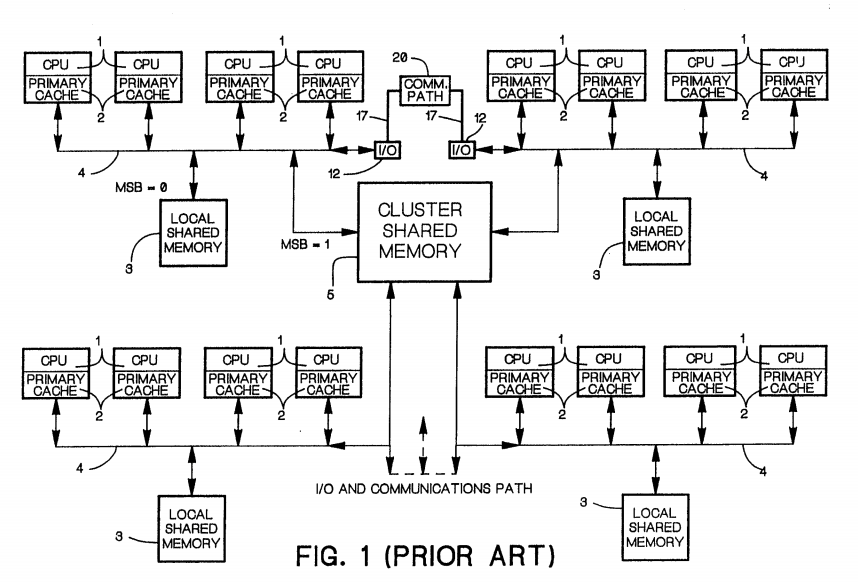
\includegraphics[scale=0.2]{cluster}
        \subcaption{Schema Computer cluster \cite{hunter1995multi}}
    \end{minipage}
    \begin{minipage}[b]{.5\linewidth}
        \centering
        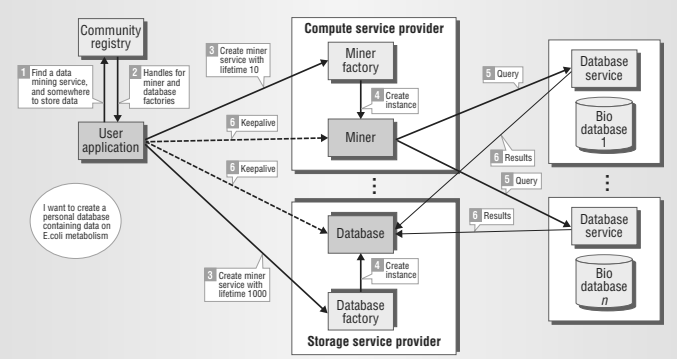
\includegraphics[scale=0.3]{grid}
        \subcaption{Schema Grid computing \cite{foster2002grid}}
    \end{minipage}
    \caption{Rappresentazione schematica del funzionamento di due architetture 
        facenti parte della categoria dell'HPC: il Computer cluster e il 
        Grid computing}
    \label{fig:cluster-grid}
\end{figure}
Per sfruttare il GPGPU è stata sfruttata la tecnologia
Computed Unified Device Architecture (CUDA) che offre la possibilità di 
sfruttare il parallelismo offerto dalle GPU moderne per ottenere incrementi 
significativi delle performance delle simulazioni effettuate su modelli di 
proliferazione cellulare riguardanti la LMA.
Durante lo sviluppo del simulatore è stato implementato l'utilizzo del 
parallelismo dinamico per simulare questi fenomeni 
di divisione cellulare inerentemente ricorsivi, trovando immediato riscontro 
positivo verificabile grazie al significativo incremento delle performance 
del simulatore. Il confronto dei dati ottenuti dalle simulazioni effettuate
tramite simulatore per CPU e dalla corrispondente versione parallela 
sviluppata durante il periodo di stage hanno confermato la correttezza dei
risultati ottenibili utilizzando la versione del software implementata con
l'ausilio della libreria CUDA.
